% chapters/ch09-case-study-clinic.tex
\chapter{Case Study: Clinic Scheduling (End-to-End)}

\begin{learningobjectives}
In this chapter you will apply the full workflow to a realistic clinic scheduling problem.
You will learn how to move from narrative to business rules, from rules to a conceptual model, and from that model to a relational schema with constraints.
You will also produce validation artifacts: key questions and a rule-to-schema traceability map.
\end{learningobjectives}

\section{Narrative}
We will intentionally keep the domain small, but realistic enough to include common modelling decisions:
identity, time, optionality, and a non-trivial business constraint.

\begin{examplebox}
\textbf{Clinic narrative}\\
A clinic has doctors and patients.
Patients book appointments with doctors.
Each appointment has a start time and a planned duration.
Appointments can be cancelled or rescheduled.
Appointments take place in rooms.
A doctor and a room cannot have overlapping scheduled appointments.
Patients may exist in the system without any appointments yet.
\end{examplebox}

The new elements here are duration, cancellation, rescheduling, and rooms.
Those elements force us to think about time, state, and shared resources.

\section{Step 1: Business rules}
Write rules as testable statements.
We will number them so they can be traced later.

\begin{examplebox}
\textbf{Business rules (clinic)}\\
R1: A patient is uniquely identified by \texttt{patient\_id}.\\
R2: A doctor is uniquely identified by \texttt{doctor\_id}.\\
R3: An appointment is with exactly one patient.\\
R4: An appointment is with exactly one doctor.\\
R5: Every appointment has a start time.\\
R6: Every appointment has a planned duration (in minutes).\\
R7: An appointment has a status in \{scheduled, cancelled\}.\\
R8: A scheduled appointment is assigned to exactly one room.\\
R9: A doctor cannot have overlapping \emph{scheduled} appointments.\\
R10: A room cannot have overlapping \emph{scheduled} appointments.\\
R11: A patient can have zero or many appointments over time.\\
R12: A doctor can have zero or many appointments over time.
\end{examplebox}

Rules R9 and R10 might look obvious, but they prevent an accidental modelling mistake:
forcing every patient/doctor to have at least one appointment.

Rule R9 is the core business constraint.
It is also a good example of a constraint that depends on time representation.
Overlaps are interval logic, not simple uniqueness.

\section{Step 2: Conceptual model}
We will model three entities: Patient, Doctor, Appointment.
Appointment is an entity rather than a mere relationship because it has its own attributes: start time, duration, and status.

\subsection{Conceptual decisions}
Before drawing anything, write the meaning in full sentences:
\begin{itemize}
  \item Each appointment belongs to exactly one patient and exactly one doctor.
  \item A patient can have many appointments; a doctor can have many appointments.
  \item Appointment has a time interval defined by (start\_time, duration).
  \item Scheduled appointments are assigned to a room; cancelled appointments do not require a room.
  \item Cancellation changes the enforcement of overlap rules: cancelled appointments do not block time.
\end{itemize}

\subsection{ER-style diagram (minimal)}
\begin{center}
\resizebox{0.95\textwidth}{!}{%
\begin{tikzpicture}[node distance=18mm]
  \erentity{EPatient}{}{Patient}{patient\_id}{name\\birth\_date}
  \erentity{EDoctor}{right=50mm of EPatient}{Doctor}{doctor\_id}{name\\specialty}
  \erentity{ERoom}{right=50mm of EDoctor}{Room}{room\_id}{name\\floor}
  \erentity{EAppt}{below=25mm of $(EPatient)!0.5!(EDoctor)$}{Appointment}{appointment\_id}{start\_time\\duration\_min\\status}

  \errel{RBooks}{below=7mm of EPatient}{books}
  \errel{RSched}{below=7mm of EDoctor}{scheduled\_with}
  \errel{RRoom}{below=7mm of ERoom}{in\_room}

  \erconnect{EPatient}{RBooks}{1}{0..N}
  \erconnect{RBooks}{EAppt}{1}{1}

  \erconnect{EDoctor}{RSched}{1}{0..N}
  \erconnect{RSched}{EAppt}{1}{1}

  \erconnect{ERoom}{RRoom}{1}{0..N}
  \erconnect{RRoom}{EAppt}{1}{1}
\end{tikzpicture}%
}
\end{center}

\begin{figure}[ht]
\centering

\includegraphics[width=0.75\textwidth]{clinic-case.pdf}
\caption{The clinic diagram highlights appointments as the event that connects patient and doctor.}
\end{figure}

This diagram does not show the overlap constraint directly.
That constraint is expressed as a business rule and later documented as a schema constraint.

\section{Step 3: Relational schema (logical, no SQL)}
Now we translate.

\subsection{Relations}
\[
\rel{Patient}(\underline{patient\_id}, name, birth\_date)
\]
\[
\rel{Doctor}(\underline{doctor\_id}, name, specialty)
\]
\[
\rel{Room}(\underline{room\_id}, name, floor)
\]
\[
\begin{aligned}
\rel{Appointment}(&\underline{appointment\_id}, start\_time, duration\_min, status, \\
&patient\_id \rightarrow \rel{Patient}, doctor\_id \rightarrow \rel{Doctor}, \\
&room\_id? \rightarrow \rel{Room})
\end{aligned}
\]

\subsection{Attribute notes}
We choose:
\begin{itemize}
  \item \texttt{duration\_min} as an integer, representing the planned duration.
  \item \texttt{status} as an attribute with a small allowed set.
  \item \texttt{room\_id} as optional, but required when status is scheduled.
\end{itemize}

In a later implementation chapter, status could also be modelled as a reference to a \rel{Status} lookup entity.
For now, we keep it as a constrained attribute.

\subsection{Constraints (conceptual specification)}
Constraints are written as statements, independent of SQL.

\begin{examplebox}
\textbf{Constraints (clinic)}\\
C1: Patient.patient\_id is unique and mandatory.\\
C2: Doctor.doctor\_id is unique and mandatory.\\
C3: Room.room\_id is unique and mandatory.\\
C4: Appointment.patient\_id references an existing Patient and is mandatory.\\
C5: Appointment.doctor\_id references an existing Doctor and is mandatory.\\
C6: Appointment.room\_id references an existing Room when status = scheduled.\\
C7: Appointment.start\_time is mandatory.\\
C8: Appointment.duration\_min is mandatory and positive.\\
C9: Appointment.status is in \{scheduled, cancelled\}.\\
C10: For each doctor, scheduled appointments must not overlap in time.\\
C11: For each room, scheduled appointments must not overlap in time.
\end{examplebox}

Constraint C9 is the key business constraint.
It is not a simple uniqueness constraint when time is interval-based.
It requires overlap detection between time intervals of the same doctor for appointments with status = scheduled.

\section{Step 5: Validation without SQL}

\subsection{Key questions}
These questions are chosen to test whether the schema supports essential operations.

\begin{itemize}
  \item Q1: What appointments does a patient have in a given week?
  \item Q2: What is a doctor’s schedule on a given day?
  \item Q3: Which patients have no future scheduled appointments?
  \item Q4: How many appointments did each doctor complete (scheduled, non-cancelled) in a month?
  \item Q5: Are there any overlaps among scheduled appointments for the same doctor?
  \item Q6: Which rooms are in use at a given time?
  \item Q7: Which appointments were cancelled or rescheduled this week?
\end{itemize}

If the schema cannot express these questions without duplication or unnatural structures, the model needs revision.

\subsection{Rule-to-schema traceability}
Now we justify that rules are represented.

\begin{examplebox}
\textbf{Traceability map (clinic)}\\[4pt]
\begin{tabularx}{\textwidth}{@{}lX@{}}
\toprule
Rule & Design element(s) \\
\midrule
R1 & Patient.patient\_id unique and mandatory (C1) \\
R2 & Doctor.doctor\_id unique and mandatory (C2) \\
R3, R4 & Appointment has mandatory FKs to Patient and Doctor (C4, C5) \\
R5, R6 & start\_time and duration\_min mandatory (C7, C8) \\
R7 & status domain constraint (C9) \\
R8 & scheduled appointments require room assignment (C6) \\
R9 & overlap prevention for scheduled appointments (C10) \\
R10 & room overlap prevention (C11) \\
R11, R12 & 1:N implied by FK direction and lack of uniqueness on FKs \\
\bottomrule
\end{tabularx}
\end{examplebox}

\subsection{Controlled test data (paper test)}
Try to represent these scenarios:
\begin{itemize}
  \item One doctor, two appointments on the same day, non-overlapping.
  \item A cancelled appointment that overlaps a scheduled one (should be valid).
  \item Two scheduled appointments that overlap (should be invalid by C10).
\end{itemize}

If you cannot express the invalid scenario clearly as a violation, the model is too permissive.
If you cannot express the cancelled-overlap scenario, the model is too restrictive.

\subsection{Invalid scenario dataset}
\begin{examplebox}
\textbf{Invalid dataset: overlapping room usage}\par\smallskip
\begin{tabular}{@{}lllll@{}}
\toprule
appointment\_id & start\_time & duration\_min & doctor\_id & room\_id \\
\midrule
A10 & 2026-02-05 09:00 & 60 & D1 & R1 \\
A11 & 2026-02-05 09:30 & 30 & D2 & R1 \\
\bottomrule
\end{tabular}
\end{examplebox}
Appointments A10 and A11 overlap in room R1.
This violates C11 (no overlapping scheduled appointments per room).

\begin{figure}[htbp]
\centering

\includegraphics[width=0.75\textwidth]{clinic-room-overlap.pdf}
\caption{Overlapping appointments in the same room violate the room scheduling rule.}
\end{figure}

\section{Time model and rescheduling}
We use intervals defined by (\texttt{start\_time}, \texttt{duration\_min}).
This fits real clinics where appointment lengths vary.
It also makes overlap constraints explicit.

\subsection{Discrete slots vs intervals}
If the clinic uses discrete slots (e.g., 15-minute blocks and fixed duration), then the overlap rule can be expressed as a simple uniqueness constraint on (doctor\_id, start\_time).
That is easier to enforce.

Intervals are more expressive, but enforcement requires overlap logic.
The modelling lesson is that representation choices affect which constraints are simple and which are complex.

\subsection{Rescheduling and cancellation}
Rescheduling is treated as changing \texttt{start\_time} and \texttt{duration\_min}.
We do not keep historical changes in this model.
If history is required, a separate \rel{AppointmentChange} entity would be appropriate.

Cancellation keeps the appointment but changes its status.
Cancelled appointments do not block time or room usage.

\section{Common mistakes}
Clinic models fail in predictable ways.

Mistake: Treating room as an attribute instead of an entity.\\
Fix: Model \rel{Room} with its own identity and constraints.

Mistake: Using status to avoid overlap rules.\\
Fix: Keep overlap constraints and decide which statuses are excluded explicitly.

Mistake: Storing end time and duration inconsistently.\\
Fix: Choose one representation and derive the other if needed.

Mistake: Forgetting rescheduling rules.\\
Fix: Specify whether rescheduling overwrites or creates new records.

\section{Mini checklist}
Before you finalize the clinic model, check:
\begin{itemize}[leftmargin=*,nosep]
  \item Are appointments modelled as event entities with their own identity?
  \item Are doctor and room overlap rules explicit and testable?
  \item Is the time representation consistent (start\_time + duration)?
  \item Are cancellations represented as a status with clear semantics?
  \item Are optional room assignments limited to cancelled appointments?
  \item Do key questions cover schedules, rooms, and cancellations?
  \item Is traceability complete for all business rules?
\end{itemize}

\begin{chaptersummary}
This case study shows the full workflow in a small domain.
The model is built from a narrative, made precise through business rules, translated through disciplined mapping, and protected through constraints.
Validation is demonstrated using key questions, traceability, and paper test scenarios.
\end{chaptersummary}

\begin{exercisebox}
Extend this clinic model.
Answer in full sentences, then update the schema in book notation.
\begin{enumerate}[label=\arabic*.]
  \item Add \term{Room} and the rule: “A room cannot host overlapping scheduled appointments.”
  \item Add a rule limiting daily appointments per doctor (choose a number and justify it).
  \item Add patient contact details and decide which are unique (if any).
  \item Add an appointment “type” (consultation, exam, follow-up) and decide how to model it (attribute vs entity).
  \item Update the traceability map for your new rules.
  \item Define an invalid scenario dataset that violates a room overlap constraint and explain the violation.
  \item Write a constraint for rescheduling that prevents moving an appointment into a blocked time.
  \item Add a rule about room availability (maintenance or closure) and show where it belongs in the schema.
\end{enumerate}
\end{exercisebox}

In the next chapter we apply the same workflow to a library case study.
Notice how different events (loans, reservations, fines) change the structure and constraints.
